\documentclass[bsc,logo,twoside,fullspacing,parskip]{infthesis}
\usepackage{url}
\usepackage{graphicx}
\usepackage{appendix}

\begin{document}

\title{Parallel Massive Dataset Cleaning}
\author{Jianmeng Yu}
\course{Computer Science}
\project{4th Year Project Report}
\date{\today}

\abstract{
\pagenumbering{roman}
This project applies the decision algorithm\cite{P1} developed by Matt Pugh in 2015 on a massive parallel scale, to remove the large amount of False Positive fish detections in the Fish4Knowledge (F4K) dataset\cite{P2}, without losing too many True Positives.

Also, according to Qiqi Yu's assessed runtime\cite{P3}, the cleaning process will take more than 1000 days to complete on a 40-core machine. Simply putting the process onto parallel scale will not be sufficient, optimization of the code is also essential for making the processing more feasible.

This document describes the detail of various approach to reduce unnecessary work during pre-processing, improve the cleaning algorithm, and evaluating efficiency of different implementations of the machine learning techniques used. A more detailed roadmap this project is provided in the Chapter 1.

}

\maketitle

\section*{Acknowledgements}
I would like to thank my project supervisor, Prof. Fisher, for his constant, patient support throughout the year. Without his expert knowledge in the field, it would be impossible for me to navigate through all of the data source and prior work of the Fish4Knowledge project. 

I would also like to thank Mr. Matthew Pugh for finding out time answering my questions on the project, and precious advices on the implementation of his algorithms.

I must also extend gratitude to my friends, and my family back in China, for all their help and encouragement during my study.

\newpage

\standarddeclaration

\tableofcontents



\chapter{Introduction}

\pagenumbering{arabic}

This project applies the previous work of Matthew Pugh\cite{P1} and Qiqi Yu\cite{P3} on massive parallel scale (detail in Chapter 2), while trying to reduce the computational cost of the cleaning algorithm. The main goal of this project is to produce a cleaned subset of a 1.6 TB dataset for future researchers.

\section{Document Structure}

Chapter 2 discussed backgrounds of the difficulties, and some of the solutions involved.

Chapter 3 described the details of the data sources, storage and preprocessing used in the cleaning algorithm.

Chapter 4 describes the first stages of the cleaning: early detection removal, feature extraction, preprocessing for classification in the next stage.

Chapter 5 discusses the final classifiers used in the cleaning, with evaluation of the results and comparison between different algorithms. 

Chapter 6 contains the conclusions and possible future work needed for the project.

\section{Fish4Knowledge Data Set}

The Fish4Knowledge (F4K) project, funded by EU's Seventh Framework Programme (FP7), studies environmental effects by analysing raw videos and extract information about observed fishes from it, so researchers could use it for studies without much programming skills. 

The project acquired video data collected by Taiwan Ocean Research Institute, they set up 9 cameras in different coral reef areas such as Nanwan National Park (NPP), Lanyu, and Houbi Lake (HoBiHu) in Taiwan. 
After 5 years of filming, the project recorded about 524,000 10-minute video clips, with a total size of 91 TB, and approximately 1.4 billion fish detection were found in the videos, we call this the F4K Original Data Set (FDS).

%TODO ask Bob who extracted these.
In attempt to reduce the dataset, F4K project developed and applied a species recognition algorithm, which extracts all detections as 100x100 RGB images and it's description files, reducing to approximately 839 million detections. These summary files have a combined size of 1.6 TB, this is called Reduced FDS (RDS), more detailed composition of these are described in Chapter \ref{sec:datasource}.

The above reduction get rids of some of the False Positives (object that are not fish, recognized as fish) from FDS, unfortunately, there are still a lot of False Positives, a classification schema is created to identify the detections.

\section{Classification Schema}
\label{sec:schema}

According to previous work of Matthew, 10 different classes were used to mark the training dataset, and later used in different classifiers for fitting. 
Fig \ref{fig:classes} shows manually picked example from each of these classes.

The classes can be divided into 3 main categories:

\renewcommand{\labelenumi}{\Roman{enumi}}
\renewcommand{\labelenumii}{\arabic{enumii}}
\renewcommand{\labelenumiii}{\roman{enumiii}}
\begin{enumerate}
 \item Not A Fish - These detection are marked for removal in future.
 \begin{enumerate}
   \item Compression Artefact - During the process of recording video, some bits were dropped during transmission of the compressed video. These detection usually have a rigid square shape.
   \item Illumination Artefact - Lighting changes recognized as fishes, some are caused by refraction of turbid water, some are caused by light reflecting planktons.
   \item Background Vegetation - Some of the video are captured with dynamic background, where the swaying plants are recognized as fishes.
   \item Others - Everything else, this includes large floating matters, empty contours created by previous algorithms.
   \item Unknown - Because of reasons like lighting and stretched video frames, it's uncertain the detection is fish or not.
 \end{enumerate}
 
 \item A Fish - These frames are useful for future researchers.
 \begin{enumerate}
   \setcounter{enumii}{5} 
   \item Good Boundary - With clear ocean as background, these fishes have good boundaries, and is useful for future species recognition.
   \item Partial Fish - Mostly good detection boundary, but part of the fish is cut-off for various reasons.
    \begin{enumerate}
      \item Fishes cut by frame boundaries.
      \item Fishes are covered by vegetation or other fishes.
      \item The fish is too big for the 100x100 boundary.
    \end{enumerate}
   \item Bad Boundary - The fish is clearly captured, but the boundary extracted is useless for research. 
 \end{enumerate}
 
 \item A Fish, but not useful - These frames detects fishes correctly, but misleading information may be extracted, it's unsure these frames should be kept or not.
 \begin{enumerate}
   \setcounter{enumii}{8} 
   \item Other Errors - like compression artefact are found in the image.
   \item Multiple Fish with shared contour.
 \end{enumerate}
\end{enumerate}

%TODO change class 9 image.
\begin{figure}[!b]
    \centering
    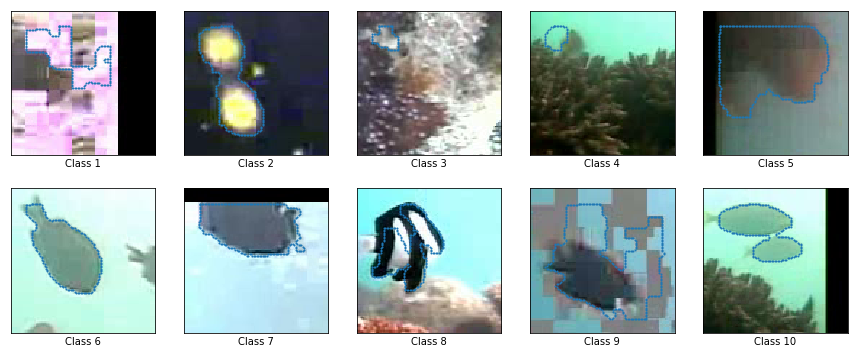
\includegraphics[scale=0.44]{graph/class_sample.png}
    \caption{Example Detection From Each Class}
    \label{fig:classes}
\end{figure}

\section{Pipeline Classifier}

\begin{figure}[!b]
    \centering
    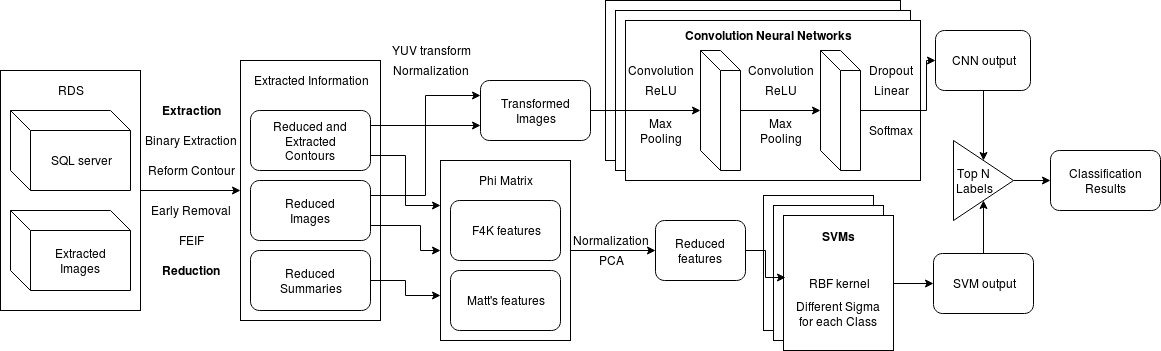
\includegraphics[scale=0.34]{graph/Pipeline_Classifier.png}
    \caption{Pipeline Classifier designed by Matthew, modified}
    \label{fig:pipeline}
\end{figure}

\chapter{Background}


\section{Big Data}

chui bi

chui bi
chui bi

\section{Message Passing Interface (MPI)}

\chapter{Data Source}
\label{sec:datasource}

from each 10 minute clip, and compiles it into a different avi file and an associated text file for description.

Under limitations of disk space and access speed, loading a large SQL database dump file into server and performing 400,000 queries is very unnecessary and time consuming, hence making it the slowest part of the cleaning.
Since each record needed for the cleaning are independent, an alternative is to use python script with stdin/out pipeline to parse and partition the dump file directly into usable csv files.
\section{Extracted Images}
\label{sec:summaries}

\section{SQL dump file}
\subsection{Stdin based Script}

\chapter{Preprocessing}

\section{Early Video Removal}

\begin{figure}
\centering
    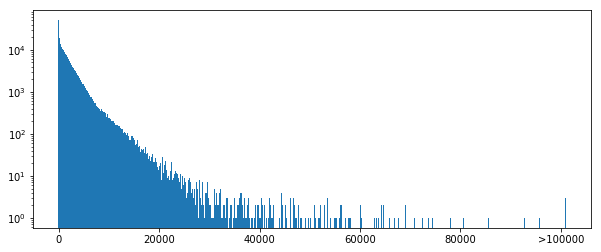
\includegraphics[scale=0.6]{graph/frame_distribution.png}
    \caption{Log Scale Histogram of Detection Length}
    \label{fig:vidlength}
\end{figure}

During the feature extraction tests, it is discovered that loading a 40,000 frame video and extract features from it would take about 8 GB of memory space, if such video is processed on a node with RAM less than 8 GB, it will cause serious thrashing, rendering the node unresponsive.  

While risking the chance of thrashing, these video took longer time to process, and most importantly, they are usually filled with False Positive detections. As discussed in Chapter \ref{sec:summaries}, if a camera recorded 30,000 detection in 10 minute, means that in every frame of the original video, an average of 10 detection is extracted. By looking into these "outlier" videos, some patterns were found:

\begin{itemize}
\item
Both Camera at Lanyu site are night-vision cameras, when they film during the night, a lot of light reflecting planktons close to the camera are recognised as fishes. Videos filmed during night have an average of 6974 detections. A 5\% of the total detection comes from such videos, with the high False Positive rate, these videos can be safely excluded from cleaning.
\item
Videos full of compression/transmission errors, mostly happens at NPP-3 site camera 2 during June 2012 to August 2012. The camera seems to be falling down and change angles every few days. Even if there are no such errors, most of the detections are from moving background vegetation.
\item
One outlier video with 200,000 detection, consists of lots of repeating frames, possibly caused by previous extraction processes.
\end{itemize}
There are also some good video with high detections: 
\begin{itemize}
\item
Videos from NPP-3 site camera 3, at January 2010. These videos are captured at a higher frame rate, resulting in more detections. They usually contains lots of good detections.
\item
Videos filled with moving vegetation, or refraction of sunlight. They usually contains lots of good detections.
\end{itemize}

Using the above patterns, if we remove all the videos recorded in the night, videos with 40,000 or more frames, and video recorded with above characteristics and 20,000 or more frames. About 8\% of the detections can be rejected without need to extract them, saving approximately 200 days of computational time.

%TODO remove me
\newpage

\section{Frame Edge Indicator Function}

what the fuck man

\section{Feature Extraction}

\subsection{F4K and Matt Feature}

\subsection{Translation Attempt}

\subsection{PCA Analysis}

\section{Image Processing For CNN}


\chapter{Classifiers}

\chapter{Conclusion}


% use the following and \cite{} as above if you use BibTeX
% otherwise generate bibtem entries
\bibliographystyle{unsrt}
\bibliography{dissertation}


\begin{appendices}
\chapter{Sample of Lengthy Videos}
%TODO say something
The videos below are some sample frames

\begin{figure}
\centering
    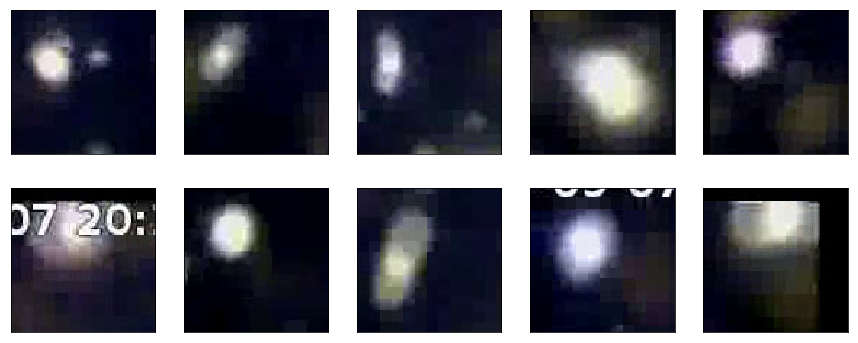
\includegraphics[scale=0.46]{graph/sample_night.png}
    \caption{Sample frames from a video filmed at night.}
    \label{fig:sample_night}
\end{figure}

\begin{figure}
\centering
    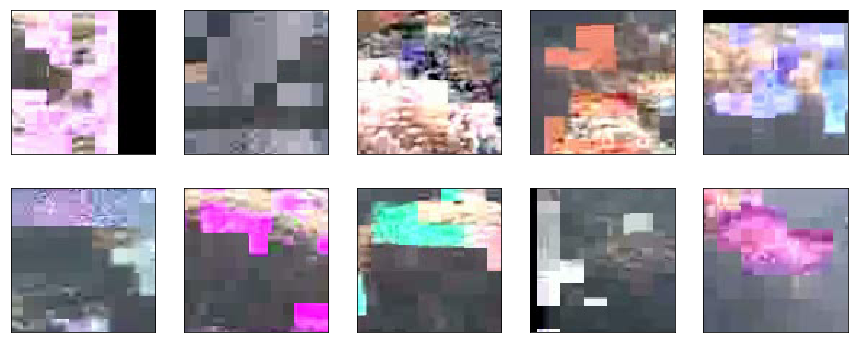
\includegraphics[scale=0.46]{graph/sample_corrupt.png}
    \caption{Sample frames from a corrupted video.}
    \label{fig:sample_corrupt}
\end{figure}

\begin{figure}
\centering
    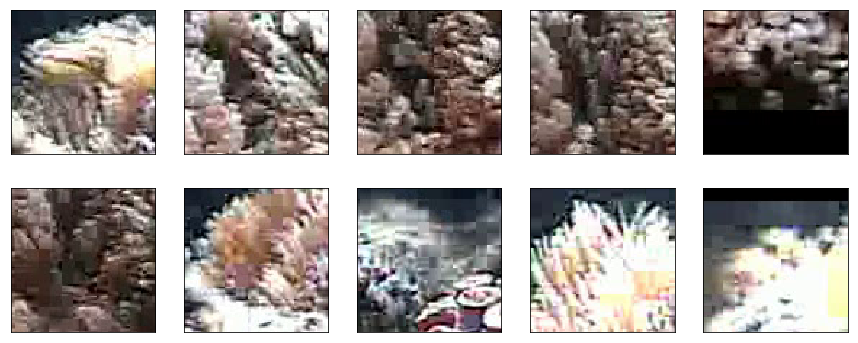
\includegraphics[scale=0.46]{graph/sample_vegetation.png}
    \caption{Sample frames from a video facing ground.}
    \label{fig:sample_vegetation}
\end{figure}
\begin{figure}
\centering
    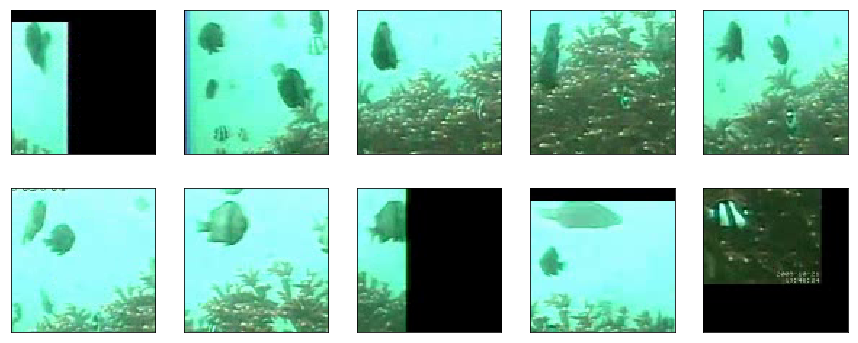
\includegraphics[scale=0.46]{graph/sample_fish.png}
    \caption{Sample frames from a video with abnormal amount of fish.}
    \label{fig:sample_fish}
\end{figure}
\end{appendices}

\end{document}